\documentclass[12pt,oneside,a4paper]{book}
\usepackage[slovak,english]{babel}
\usepackage[utf8]{inputenc}
\usepackage[T1]{fontenc}
\usepackage{graphicx}
\usepackage{float}
\usepackage[pdftex,bookmarks=true]{hyperref}
\usepackage[right=2.0cm,left=3.5cm,top=2.5cm,bottom=2.5cm]{geometry}
\usepackage{listings}
\usepackage{color}

\linespread{1.3} %riadkovanie 1.5

%%%%%%%%%%%%%%%%%%%%%%%%%%%%%%%%%%%%%%%%%%%%%%%%%%%%%%%%%%%%%%%%%%%%%%%%%%%%%%%
% Základne údaje o práci
%%%%%%%%%%%%%%%%%%%%%%%%%%%%%%%%%%%%%%%%%%%%%%%%%%%%%%%%%%%%%%%%%%%%%%%%%%%%%%%
\def\university{Univerzita Komenského v Bratislave}
\def\faculty{Faculta matematiky, fyziky a informatiky}
\def\title{Science Background of the Lorem Ipsum}
\def\thesis{Bakalárka práca}
\def\author{Jožko Mrkvička}
\def\year{2014}
\def\placeandyear{Bratislava, \year}
\def\supervisor{RNDr. Kleofáš Učený, PhD.\ }
\def\studyprogramme{Aplikovaná informaitka}
\def\studyfield{9.2.1 Aplikovaná informatika}
\def\department{Katedra aplikovanej informatiky}

\pdfinfo{/Author (\author) /Title (\title)}

\begin{document}

\selectlanguage{slovak}

% Colors
\definecolor{javareserved}{RGB}{0, 0, 255}
\definecolor{javacomment}{gray}{0.6}
\definecolor{javabg2}{gray}{0.6}
\definecolor{javabg}{gray}{0.98}

% Listings Java configuration
\lstset{language=Java}
\lstset{columns=flexible}
\lstset{basicstyle=\small\ttfamily}
\lstset{sensitive=true}
\lstset{morestring=[b]}
\lstset{string=[b]}
\lstset{commentstyle=\itshape\color{javacomment}}
\lstset{backgroundcolor=\color{javabg}}
\lstset{numberstyle=\color{flexred}}
\lstset{numberblanklines=true}
\lstset{breaklines=true}
\lstset{frame=l}
\lstset{framerule=6pt}
\lstset{rulecolor=\color{javabg2}}
\lstset{framexleftmargin=0pt}
\lstset{emph =
       {[2]
abstract,else,interface,super,
boolean,extends,long,switch,
break,final,native,synchronized,
byte,finally,new,this,
case,float,package,throw,
catch,for,private,throws,
char,if,protected,transient,
class,implements,public,try,
continue,import,return,void,
default,instanceof,short,volatile,
do,int,static,while,
double,var,HSTREAM,begin,end
       }}
\lstset{emphstyle={[2]\color{javareserved}\textbf}}


%%%%%%%%%%%%%%%%%%%%%%%%%%%%%%%%%%%%%%%%%%%%%%%%%%%%%%%%%%%%%%%%%%%%%%%%%%%%%%%
% Úvodná strana
%%%%%%%%%%%%%%%%%%%%%%%%%%%%%%%%%%%%%%%%%%%%%%%%%%%%%%%%%%%%%%%%%%%%%%%%%%%%%%%
\frontmatter
\pagestyle{empty}
\begin{minipage}{0.20\textwidth}

\includegraphics[width=0.9\textwidth]{images/comenius_university_logo}
\end{minipage}
\begin{minipage}{0.79\textwidth}
\begin{center}
\sc \department\\
\faculty\\
\university\\
\end{center}
\end{minipage}

\vfill
\begin{center}
\begin{minipage}{0.8\textwidth}
\hrule
\bigskip\bigskip
\begin{center}
{\LARGE\sc \title}
\end{center}
\smallskip
\centerline{(\thesis)}
\bigskip
\bigskip
\centerline{\large\sc \author}
\bigskip\bigskip
\hrule
\end{minipage}
\end{center}

\vfill
\begin{flushleft}
  \begin{tabular}{@{}ll}
    Študjný program: & \studyprogramme \\
    Študjný odbor: & \studyfield \\
    Školiace pracovisko: & \department \\
    Školiteľ: & \supervisor
  \end{tabular}
  \vspace{1cm}

  \placeandyear\\
\end{flushleft}

%%%%%%%%%%%%%%%%%%%%%%%%%%%%%%%%%%%%%%%%%%%%%%%%%%%%%%%%%%%%%%%%%%%%%%%%%%%%%%%
% Čestné prehlásenie 
%%%%%%%%%%%%%%%%%%%%%%%%%%%%%%%%%%%%%%%%%%%%%%%%%%%%%%%%%%%%%%%%%%%%%%%%%%%%%%%
\newpage
\begin{minipage}{1.00\textwidth}
\vspace{15.6cm}
Čestne prehlasujem, že som túto prácu vypracoval samostatne s použitím citovaných
zdrojov.
\hfill\hbox to 6cm{\dotfill}
\end{minipage}

%%%%%%%%%%%%%%%%%%%%%%%%%%%%%%%%%%%%%%%%%%%%%%%%%%%%%%%%%%%%%%%%%%%%%%%%%%%%%%%
% Poďakovanie
%%%%%%%%%%%%%%%%%%%%%%%%%%%%%%%%%%%%%%%%%%%%%%%%%%%%%%%%%%%%%%%%%%%%%%%%%%%%%%%
\newpage
\chapter*{Poďakovanie}
\vfil
Chcel by som poďakovať školiteľovi \ldots

%%%%%%%%%%%%%%%%%%%%%%%%%%%%%%%%%%%%%%%%%%%%%%%%%%%%%%%%%%%%%%%%%%%%%%%%%%%%%%%
% Abstrakt SK
%%%%%%%%%%%%%%%%%%%%%%%%%%%%%%%%%%%%%%%%%%%%%%%%%%%%%%%%%%%%%%%%%%%%%%%%%%%%%%%
\chapter*{Abstrakt}
Zhrnutie práce v slovenskom jazyku.

\textbf{Kľúčové slová:}

%%%%%%%%%%%%%%%%%%%%%%%%%%%%%%%%%%%%%%%%%%%%%%%%%%%%%%%%%%%%%%%%%%%%%%%%%%%%%%%
% Abstrakt EN
%%%%%%%%%%%%%%%%%%%%%%%%%%%%%%%%%%%%%%%%%%%%%%%%%%%%%%%%%%%%%%%%%%%%%%%%%%%%%%%
\selectlanguage{english}
\chapter*{Abstract}
Summary of the thesis in English.

\textbf{Keywords:}

%%%%%%%%%%%%%%%%%%%%%%%%%%%%%%%%%%%%%%%%%%%%%%%%%%%%%%%%%%%%%%%%%%%%%%%%%%%%%%%
% Obsah, zoznam obrázkov a tabuliek
%%%%%%%%%%%%%%%%%%%%%%%%%%%%%%%%%%%%%%%%%%%%%%%%%%%%%%%%%%%%%%%%%%%%%%%%%%%%%%%
\selectlanguage{slovak}

\tableofcontents
\listoffigures
\listoftables

%%%%%%%%%%%%%%%%%%%%%%%%%%%%%%%%%%%%%%%%%%%%%%%%%%%%%%%%%%%%%%%%%%%%%%%%%%%%%%%
% Samotná práca
%%%%%%%%%%%%%%%%%%%%%%%%%%%%%%%%%%%%%%%%%%%%%%%%%%%%%%%%%%%%%%%%%%%%%%%%%%%%%%%
\mainmatter

\chapter{Úvod}
Úvod do problematiky.


\chapter{Prehľad problematiky}
\section{Podkapitola}

\subsection{Podkpitola podkapitoly :) }

Citacia ~\cite{Itti1998}.

Odkaz na obrazok (Obr. ~\ref{fig:yarbus}).

\begin{figure}
  \centering
    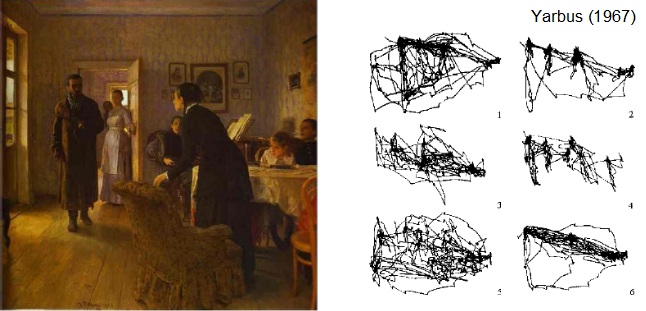
\includegraphics[width=11cm]{images/Yarbus.png}
    \caption[Kratky popis obrazka]{Obraz bol skúmaný pozorovateľom s rôznymi inštrukciami: 1) voľne pozorovať obraz 2) odhadnúť vek osôb 3) zistiť, čo robili osoby pred príchodom návštevníka 4) zapamätať si oblečenie osôb 5) zapamätať si pozíciu osôb a objektov v miestnosti  6) odhadnúť, ako dlho bol návštevník preč~\cite{Cater2003}}
  \label{fig:yarbus}
\end{figure}

\begin{equation}
     \overline{\cal{I}}  = \oplus _{c=2}^{4} \oplus _{s=c+3}^{c+4} \begin{cal}N\end{cal}(\begin{cal}I\end{cal}(c,s))
\end{equation}

\begin{equation}
    \overline{\begin{cal}C\end{cal}}  = \oplus _{c=2}^{4} \oplus _{s=c+3}^{c+4} [\begin{cal}N\end{cal}(\begin{cal}RG\end{cal}(c,s)) + \begin{cal}N\end{cal}(\begin{cal}BY\end{cal}(c,s))]
\end{equation}

\begin{table}[t]
  \centering
   \begin{tabular}{|r|c|l|}
     \hline
     stlpec 1&stlpec 1&stlpec 1\\
     \hline
     1& 1& 1\\
     2& 2& 2\\
     \hline
   \end{tabular}
   \caption{Porovnanie systémov na detekciu tváre}
  \label{tab:table1}
\end{table} 

\newpage
ukazka kodu
\begin{verbatim}
maximum_SF = max(max(SF1));
for i = 1: HEIGHT
    for j = 1 : WIDTH
   		SF(i,j) = SF1(i,j)+FACE(i,j);
    end
end
\end{verbatim}


\chapter{Záver}
Zhrnutie práce.

%%%%%%%%%%%%%%%%%%%%%%%%%%%%%%%%%%%%%%%%%%%%%%%%%%%%%%%%%%%%%%%%%%%%%%%%%%%%%%%
% Literatúra
%%%%%%%%%%%%%%%%%%%%%%%%%%%%%%%%%%%%%%%%%%%%%%%%%%%%%%%%%%%%%%%%%%%%%%%%%%%%%%%
\bibliographystyle{plain}
\bibliography{literatura}

\end{document} 
